\ifx\wholebook\relax \else
\documentclass[b5paper]{article}
\usepackage[nomarginpar
  %, margin=.5in
]{geometry}

\addtolength{\oddsidemargin}{-0.05in}
\addtolength{\evensidemargin}{-0.05in}
\addtolength{\textwidth}{0.1in}
\usepackage[en]{../../../prelude}

\setcounter{page}{1}

\begin{document}

\title{Binomial heap, Fibonacci heap, and pairing heap}

\author{Xinyu~LIU
\thanks{{\bfseries Xinyu LIU} \newline
  Email: liuxinyu95@gmail.com \newline}
  }

\maketitle
\fi

\markboth{Binomial heap, Fibonacci heap, and pairing heap}{Elementary Algorithms}

\ifx\wholebook\relax
\chapter{Binomial heap, Fibonacci heap, and pairing heap}
\numberwithin{Exercise}{chapter}
\fi

\section{Introduction}
\label{introduction}

Binary heap stores elements in a binary tree, we can extend it to $k$-ary tree\cite{K-ary-tree} ($k > 2$ multi-ways tree), or multiple trees. This chapter introduces binomial heap, which consists of forest of $k$-ary trees. When delay some operations to a Binomial heap, we obtained Fibonacci heap. It improves the heap merge performance from $O(\lg n)$ time bound to amortized constant time. This is critical for graph algorithm design. We give pairing heap as a simplified heap implementation with good overall performance.

\section{Binomial Heaps}
\label{sec:binomial-heap} \index{Binomial heap}

Binomial heap is named after Newton's binomial theorem. It consists of a set of $k$-ary trees (also called a forest). Every tree has the size equal to a binomial coefficient. Newton proved that $(a + b)^n$ expands to:

\be
(a + b)^n = a^n + \binom{n}{1} a^{n-1}b + ... + \binom{n}{n-1} a b^{n-1} + b
\ee

When $n$ is a natural number, the coefficients is some row in Pascal's triangle\footnote{Also know as the {\em Jia Xian}'s triangle named after ancient Chinese mathematician Jia Xian (1010-1070). Newton generalized $n$ to rational numbers, later Euler expand it to real exponents.}\cite{wiki-pascal-triangle}.

\begin{verbatim}
    1
   1 1
  1 2 1
 1 3 3 1
1 4 6 4 1
...
\end{verbatim}

The first row is 1, all the first and last numbers are 1 for every row. Any other number is the sum of the top-left and top-right numbers in the previous row. There are many methods to generate pascal triangles, like recursion.

\subsubsection{Binomial tree}
\label{Binomial tree} \index{Binomial tree}

A binomial tree is a multi-ways tree with an integer rank. Denoted as $B_0$ if the rank is 0, and $B_n$ for rank $n$.

\begin{enumerate}
\item $B_0$ has only one node;
\item $B_n$ is formed by two $B_{n-1}$ trees, the one with the greater root element is the left most sub-tree of the other, as shown in \cref{fig:link-bitree}.
\end{enumerate}

\begin{figure}[htbp]
  \centering
  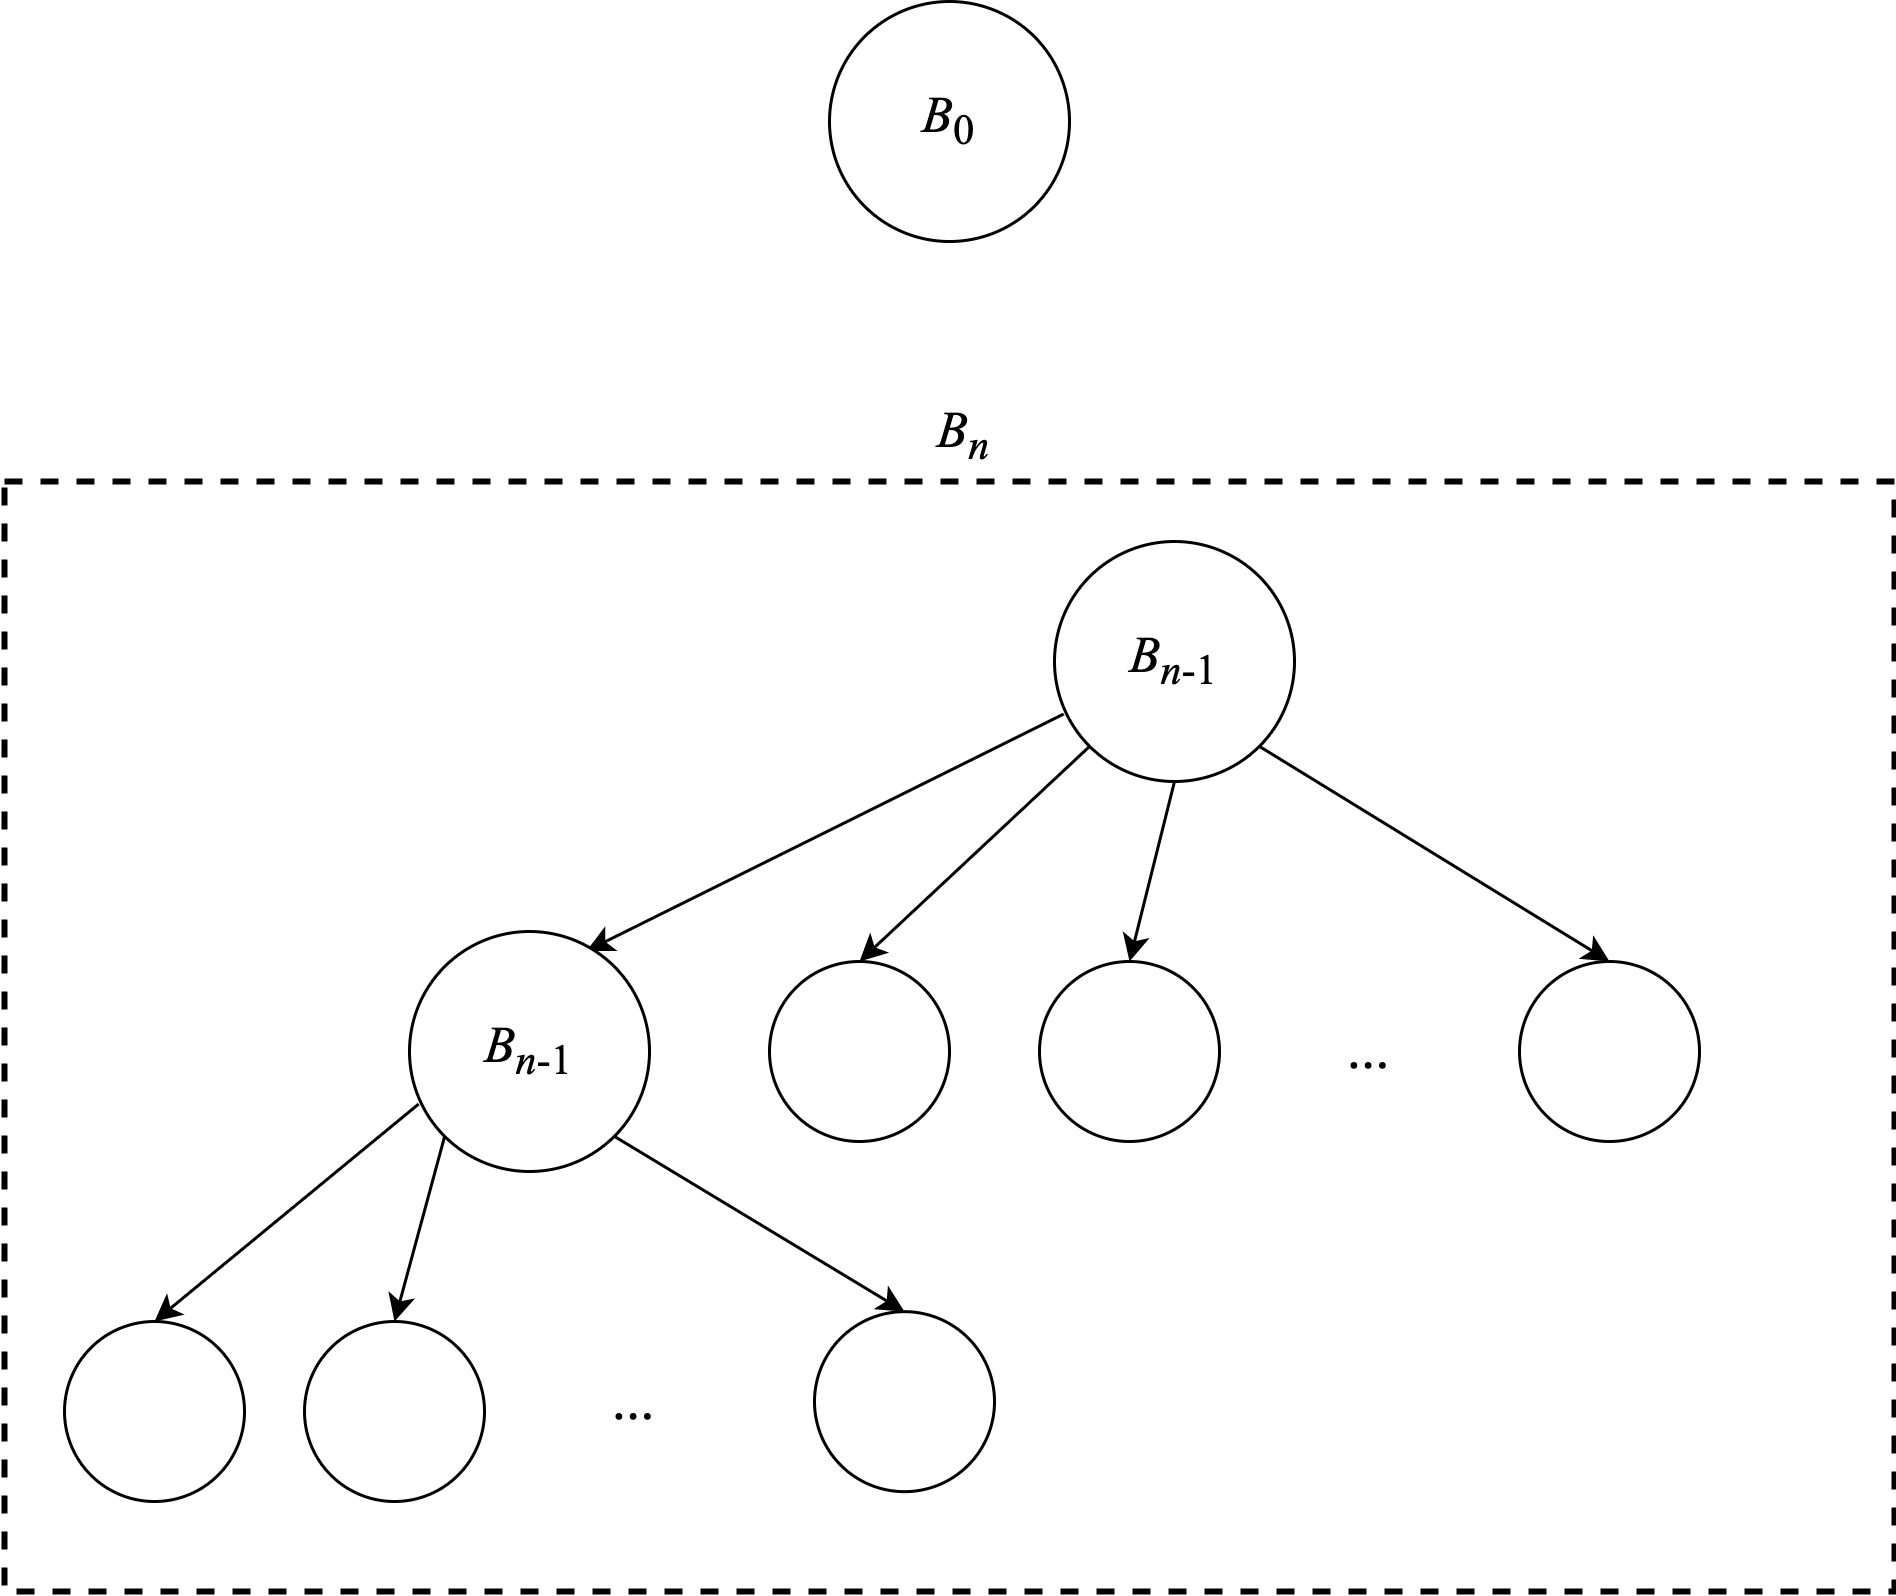
\includegraphics[scale=0.5]{img/btrees}
  \caption{Binomial tree}
  \label{fig:link-bitree}
\end{figure}

\Cref{fig:bitree-forms} gives examples of $B_0$ to $B_4$.

\begin{figure}[htbp]
  \centering
  \subcaptionbox{$B_0$}{\hspace{0.05\textwidth}\includegraphics[scale=0.5]{img/b0tree}\hspace{0.05\textwidth}}
  \subcaptionbox{$B_1$}{\hspace{0.05\textwidth}\includegraphics[scale=0.5]{img/b1tree}\hspace{0.05\textwidth}}
  \subcaptionbox{$B_2$}{\includegraphics[scale=0.5]{img/b2tree}}
  \subcaptionbox{$B_3$}{\includegraphics[scale=0.5]{img/b3tree}} \\
  \subcaptionbox{$B_4$}{\includegraphics[scale=0.5]{img/b4tree}...}
  \caption{Binomial trees of rank 0, 1, 2, 3, 4, ...}
  \label{fig:bitree-forms}
\end{figure}

We can find the number of nodes in every row in $B_n$ is a binomial coefficient. For example in $B_4$, there is a node (root) in level 0, 4 nodes in level 1, 6 nodes in level 2, 4 nodes in level 3, and a node in level 4. They are exactly same as the 4th row (start from 0) of Pascal's triangle: 1, 4, 6, 4, 1. This is the reason why we name it binomial tree. We can further know there are $2^n$ elements in a $B_n$ tree.

\label{Binomial heap} \index{Binomial heap!definition}

A binomial heap is a set of binomial trees (a forest) that satisfies the following two rules:

\begin{enumerate}
\item Every tree satisfies the {\em heap property}, i.e. for min heap, the element in every node is not less than ($\geq$) its parent;
\item Every tree has unique rank. i.e. any two trees have different ranks.
\end{enumerate}

From the 2nd rule, for a binomial heap of $n$ elements, convert $n$ to its binary format $(a_m ... a_1, a_0)_2$, where $a_0$ is the least significant bit (LSB) and $a_m$ is the most significant bit (MSB). If if $a_i=0$, there is no tree of rank $i$; if $a_i = 1$, there is a tree of rank $i$. For example, consider a binomial heap of 5 elements. As 5 is 101 in binary, there are 2 binomial trees, one is $B_0$, the other is $B_2$. The binomial heap in \cref{fig:bheap2} has 19 elements, 19 is $(10011)_2$. There is a $B_0$, a $B_1$, and a $B_4$.

\begin{figure}[htbp]
  \centering
  \includegraphics[scale=0.5]{img/bheap2}
  \caption{A binomial heap with 19 elements}
  \label{fig:bheap2}
\end{figure}

We define the binomial tree as $(r, k, ts)$, where $r$ is the rank, $k$ is the element in the root, and $ts$ is the list of sub-trees ordered by rank.

\lstset{frame=single}
\begin{Haskell}
data BiTree a = Node Int a [BiTree a]

type BiHeap a = [BiTree a]
\end{Haskell}

\index{left child, right sibling}
There is a method called `left-child, right-sibling'\cite{CLRS}, that can reuse the binary tree data structure to define multi-ways tree. Every node has the left and right part. the left references to the first sub-tree; the right references to its sibling. All siblings form a list as shown in \cref{fig:lcrs}. Alternatively, we can use an array or a list to represent the sub-trees.

\begin{figure}[htbp]
  \centering
  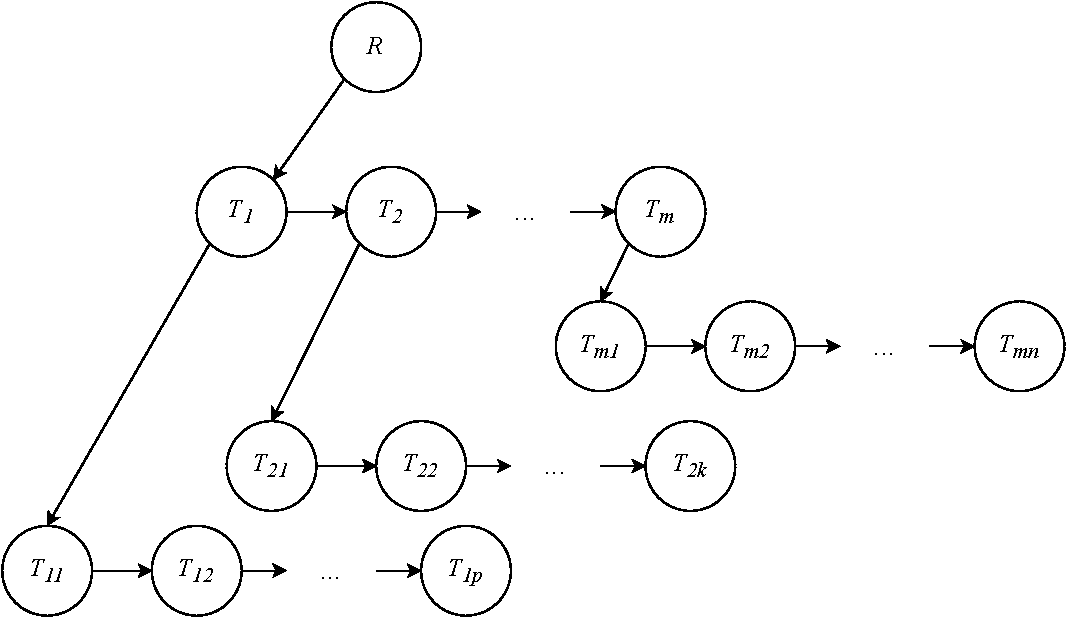
\includegraphics[scale=0.5]{img/left-child-right-sibling}
  \caption{$R$ is the root, $T_1, T_2, ..., T_m$ are sub-trees of $R$. The left of $R$ is $T_1$, the right is NIL. $T_{11}, ..., T_{1p}$ are sub-trees of $T_1$. The left of $T_1$ is $T_{11}$, the right is its sibling $T_2$. The left of $T_2$ is $T_{21}$, the left is sibling.}
  \label{fig:lcrs}
\end{figure}

\subsection{Link}
\index{Binomial Heap!Link}

To link two $B_n$ trees to a $B_{n+1}$ tree, we compare the two root elements, choose the smaller one as the root, and put the other tree ahead of other sub-trees as shown in \cref{fig:link-xy}.

\be
link\ (r, x, ts)\ (r, y, ts') = \begin{cases}
  x < y: & (r + 1, x, (r, t, ts') : ts) \\
  \text{otherwise}: & (r + 1, y, (r, x, ts): ts') \\
  \end{cases}
\label{eq:link}
\ee

\begin{figure}[htbp]
  \centering
  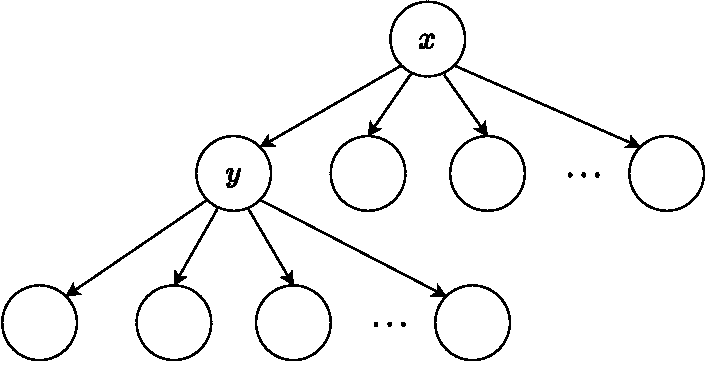
\includegraphics[scale=0.5]{img/link-bitree-xy}
  \caption{If $x < y$, link $y$ as the first sub-tree of $x$.}
  \label{fig:link-xy}
\end{figure}

We can implement link with `left child, right sibling' method as below. Link operation is bound to constant time.

\begin{algorithmic}[1]
\Function{Link}{$x, y$}
  \If{\Call{Key}{$y$} $<$ \Call{Key}{$x$}}
    \State Exchange $x \leftrightarrow y$
  \EndIf
  \State \Call{Sibling}{$y$} $\gets$ \Call{Sub-Trees}{$T_1$}
  \State \Call{Sub-Trees}{$x$} $\gets y$
  \State \Call{Parent}{$y$} $\gets x$
  \State \Call{Rank}{$x$} $\gets$ \Call{Rank}{$y$} + 1
  \State \Return $x$
\EndFunction
\end{algorithmic}

\begin{Exercise}\label{ex:binomial-tree}
\Question{Write a program to generate Pascal's triangle.}
\Question{Prove that the $i$-th row in tree $B_n$ has $\binom{n}{i}$ nodes.}
\Question{Prove there are $2^n$ elements in $B_n$ tree.}
\Question{Use a container to store sub-trees, how to implement link? How to secure the operation is in constant time?}
\end{Exercise}

\begin{Answer}[ref = {ex:binomial-tree}]
\Question{Write a program to generate Pascal's triangle.
\begin{Haskell}[frame=single]
pascal = gen [1] where
  gen cs (x:y:xs) = gen ((x + y) : cs) (y:xs)
  gen cs _ = 1 : cs
\end{Haskell}
}
\Question{Prove that the $i$-th row in tree $B_n$ has $\binom{n}{i}$ nodes.
\begin{proof}
Use induction. There is only a root node for $B_0$. Assume every row in $B_n$ is binomial number. Tree $B_{n+1}$ is composed from two $B_n$ trees. The 0-th row contains root: $1 = \binom{n+1}{0}$. The $i$-th row has two parts: one from the $(i-1)$-th row of the left most sub-tree $B_n$, the other from the $i$-th row of the other $B_n$ tree. In total:

\[
\begin{array}{rcl}
\binom{n}{i-1} + \binom{n}{i} & = & \dfrac{n!}{(i-1)!(n-i+1)!} + \dfrac{n!}{i!(n-i)!} \\
 & = & \dfrac{n!}{(i-1)!(n-i)!}(\dfrac{1}{i} - \dfrac{1}{n-i+1}) \\
 & = & \dfrac{n!}{(i-1)!(n-i)!}\dfrac{n+1}{i(n-i+1)} \\
 & = & \dfrac{(n+1)!}{i!(n-i+1)!} \\
 & = & \binom{n+1}{i} \\
\end{array}
\]
\end{proof}
}
\Question{Prove there are $2^n$ elements in $B_n$ tree.
\begin{proof}
From previous exercise, sum all rows of $B_n$ tree:
\[
\begin{array}{cll}
  & \binom{n}{0} + \binom{n}{1} + ... + \binom{n}{n} & \text{Sum rows} \\
= & (1 + 1)^n & \text{Let}\ a = b = 1\ \text{in}\ (a + b)^n \\
= & 2^n & \\
\end{array}
\]
\end{proof}
}
\Question{Use a container to store sub-trees, how to implement link? How to secure the operation is in constant time?
If store all sub-trees in an array, we need linear time to insert a new tree ahead of all sub-trees:

\begin{algorithmic}[1]
\Function{Link'}{$T_1, T_2$}
  \If{\Call{Key}{$T_2$} $<$ \Call{Key}{$T_1$}}
    \State Exchange $T_1 \leftrightarrow T_2$
  \EndIf
  \State \Call{Parent}{$T_2$} $\gets T_1$
  \State \textproc{Insert}(\Call{Sub-Trees}{$T_1$}, 1, $T_2$)
  \State \Call{Rank}{$T_1$} $\gets$ \Call{Rank}{$T_2$} + 1
  \State \Return $T_1$
\EndFunction
\end{algorithmic}

We can store the sub-trees in reversed order, it's need constant time to append the new tree on tail.
}
\end{Answer}

\subsubsection{Insert}
\index{Binomial heap!insert} \index{Binomial heap!push}

When insert a new tree, we keep the trees in binomial heap ordered by rank (ascending):

\be
\begin{array}{rcl}
ins\ t\ [\ ] & = & [t] \\
ins\ t\ (t':ts) & = & \begin{cases}
  rank\ t < rank\ t': & t:t':ts \\
  rank\ t' < rank\ t: & t' : ins\ t\ ts \\
  \text{otherwise}: & ins\ (link\ t\ t')\ ts  \\
\end{cases}
\end{array}
\ee

Where $rank\ (r, k, ts) = r$ gives the rank of a tree. For empty heap $[\ ]$, it becomes a single list of the new tree $t$; otherwise, we compare the rank of $t$ with the first tree $t'$, if $t$ has less rank, then it becomes the new first one; if $t'$ has less rank, we recursively insert $t$ to the rest trees; if they have the same rank, then link $t$ and $t'$ to a bigger tree, and recursively insert to the rest. For $n$ elements, there are at most $O(\lg n)$ binomial trees in the heap. $ins$ links $O(\lg n)$ time at most, as linking is bound to constant time, the overall performance is bound to $O(\lg n)$\footnote{It's similar to adding two binary numbers. A more generic topic is {\em numeric representation}\cite{okasaki-book}.}. We can define insert for binomial heap with $ins$. First wrap the new element $x$ in a singleton tree, then insert the tree to the heap:

\be
insert\ x = ins\ (0, x, [\ ])
\ee

This is a Curried definition, we can further insert a list of elements to the heap by using fold:

\be
\textit{fromList} = foldr\ insert\ [\ ]
\ee

Below is the implementation with 'left child, right sibling' method: \label{alg:insert-tree}

\begin{algorithmic}[1]
\Function{Insert-Tree}{$T, H$}
  \State $\perp \gets p \gets$ \Call{Node}{$0$, NIL, NIL}
  \While{$H \neq$ NIL 且 \Call{Rank}{$H$} $\leq$ \Call{Rank}{$T$}}
    \State $T_1 \gets H$
    \State $H \gets $ \Call{Sibling}{$H$}
    \If{\Call{Rank}{$T$} = \Call{Rank}{$T_1$}}
      \State $T \gets$ \Call{Link}{$T, T_1$}
    \Else
      \State \Call{Sibling}{$p$} $\gets T_1$
      \State $p \gets T_1$
    \EndIf
  \EndWhile
  \State \Call{Sibling}{$p$} $\gets T$
  \State \Call{Sibling}{$T$} $\gets H$
  \State \Return \Call{Remove-First}{$\perp$}
\EndFunction
\Statex
\Function{Remove-First}{$H$}
  \State $n \gets$ \Call{Sibling}{$H$}
  \State \Call{Sibling}{$H$} $\gets$ NIL
  \State \Return $n$
\EndFunction
\end{algorithmic}

\subsection{Merge}
\index{Binomial tree!merge}

When merge two binomial heaps, we actually merge two lists of binomial trees. Every tree has unique rank in merged result, and the ranks are in ascending order. The tree merge process is similar to merge sort. Every time, we pick the first tree from each heap, compare their ranks, put the smaller one to the result. If the two trees have the same rank, we link them to a bigger one, and recursively insert to the merge result.

\be
\begin{array}{rcl}
merge\ ts_1\ [\ ] & = & ts_1 \\
merge\ [\ ]\ ts_2 & = & ts_2 \\
merge\ (t_1:ts_1)\ (t_2:ts_2) & = & \begin{cases}
  rank\ t_1 < rank\ t_2: & t_1 : (merge\ ts_1\ (t_2:ts_2)) \\
  rank\ t_2 < rank\ t_1: & t_2 : (merge\ (t_1:ts_1)\ ts_2) \\
  \text{otherwise}: & ins\ (link\ t_1\ t_2)\ (merge\ ts_1\ ts_2) \\
  \end{cases}
\end{array}
\ee

Alternatively, when $t_1$ and $t_2$ have the same rank, we can insert the linked tree back to either heap, and recursively merge:

\[
merge\ (ins\ (link\ t_1\ t_2)\ ts_1)\ ts_2
\]

We can also eliminate recursion, and implement iterative merge:

\begin{algorithmic}[1]
\Function{Merge}{$H_1, H_2$}
  \State $H \gets p \gets$ \Call{Node}{0, NIL, NIL}
  \While{$H_1 \neq$ NIL and $H_2 \neq$ NIL}
    \If{\Call{Rank}{$H_1$} $<$ \Call{Rank}{$H_2$}}
      \State \Call{Sibling}{$p$} $\gets H_1$
      \State $p \gets$ \Call{Sibling}{$p$}
      \State $H_1 \gets$ \Call{Sibling}{$H_1$}
    \ElsIf{\Call{Rank}{$H_2$} $<$ \Call{Rank}{$H_1$}}
      \State \Call{Sibling}{$p$} $\gets H_2$
      \State $p \gets$ \Call{Sibling}{$p$}
      \State $H_2 \gets$ \Call{Sibling}{$H_2$}
    \Else \Comment{same rank}
      \State $T_1 \gets H_1, T_2 \gets H_2$
      \State $H_1 \gets$ \Call{Sibling}{$H_1$}, $H_2 \gets$ \Call{Sibling}{$H_2$}
      \State $H_1 \gets $ \textproc{Insert-Tree}(\Call{Link}{$T_1, T_2$}, $H_1$)
    \EndIf
  \EndWhile
  \If{$H_1 \neq$ NIL}
    \State \Call{Sibling}{$p$} $\gets H_1$
  \EndIf
  \If{$H_2 \neq$ NIL}
    \State \Call{Sibling}{$p$} $\gets H_2$
  \EndIf
  \State \Return \Call{Remove-First}{$H$}
\EndFunction
\end{algorithmic}

If there are $m_1$ trees in $H_1$, $m_2$ trees in $H_2$. There are at most $m_1 + m_2$ trees after merge. The merge is bound to $O(m_1 + m_2)$ time if all trees have different ranks. If there exist trees of the same rank, we call $ins$ up to $O(m_1 + m_2)$ times. Consider $m_1 = 1 + \lfloor \lg n_1 \rfloor$ and $m_2 = 1 + \lfloor \lg n_2 \rfloor$, where $n_1$, $n_2$ are the numbers of elements in each heap, and $\lfloor \lg n_1 \rfloor + \lfloor \lg n_2 \rfloor \leq 2 \lfloor \lg n \rfloor$, where $n = n_1 + n_2$. The final performance of merge is $O(\lg n)$.

\subsubsection{Pop}
\index{Binomial heap!pop}

Although every tree has the minimal element in its root, we don't know which tree holds the overall minimum in the heap. We need locate it from all trees. As there are $O(\lg n)$ trees, it takes $O(\lg n)$ time to find the top element. For pop, we need further remove the top element and maintain heap property. Let the trees be $B_i, B_j, ..., B_p, ..., B_m$ in the heap, and the minimum is in the root of $B_p$. After remove the top, there leave $p$ sub binomial trees with ranks of $p-1, p-2, ..., 0$. We can reverse them to form a new binomial heap $H_p$. The other trees without $B_p$ also form a binomial heap $H' = H - [B_p]$. We merge $H_p$ and $H'$ to get the final result as shown in \cref{fig:bheap-del-min}. Below is the definition to access the minimal element in the heap.

\begin{figure}[htbp]
  \centering
  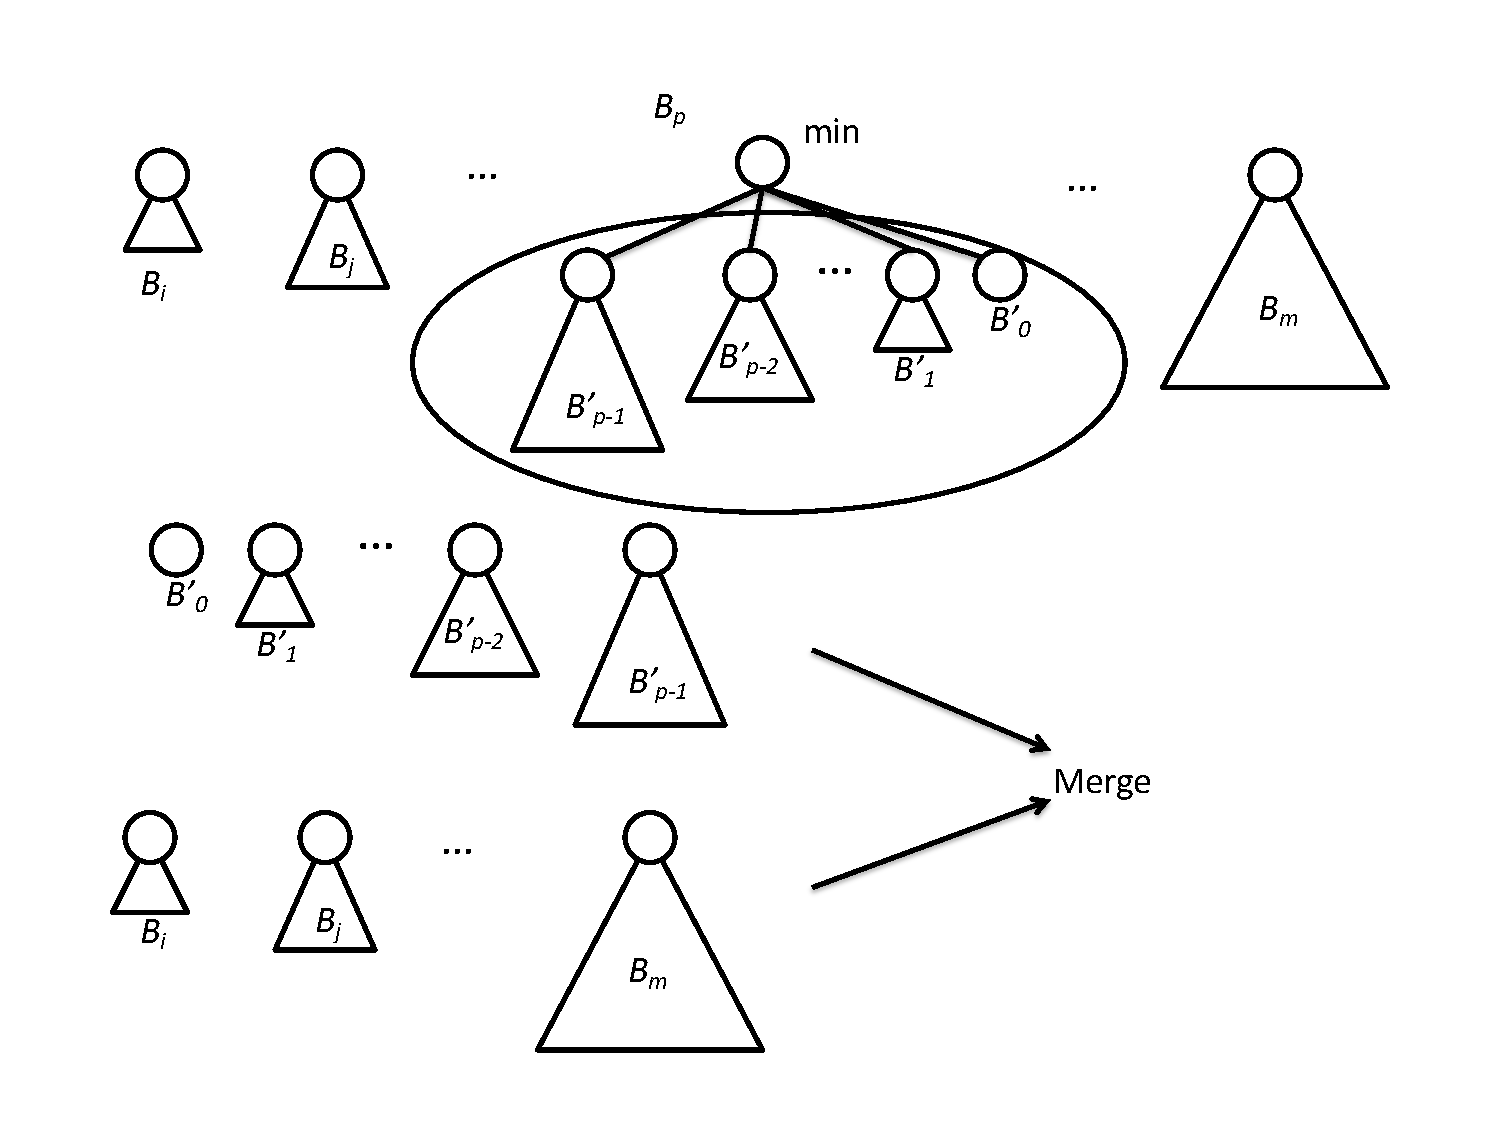
\includegraphics[scale=0.4]{img/bheap-pop}
  \caption{Binomial heap pop.}
  \label{fig:bheap-del-min}
\end{figure}

\be
top\ (t:ts) = foldr\ f\ (key\ t)\ ts
\ee

\[
f\ (r, x, ts)\ y = min\ x\ y
\]

It's means to traverse all trees and find the which root has the minimum.

\begin{algorithmic}[1]
\Function{Top}{$H$}
  \State $m \gets \infty$
  \While{$H \neq$ NIL}
    \State $m \gets$ \textproc{Min}($m$, \Call{Key}{$H$})
    \State $H \gets $ \Call{Sibling}{$H$}
  \EndWhile
  \State \Return $m$
\EndFunction
\end{algorithmic}

To support pop, we need extract the tree containing the minimum out:

\be
\begin{array}{rcl}
min'\ [t] & = & (t, [\ ]) \\
min'\ (t:ts) & = & \begin{cases}
  key\ t < key\ t': & (t, ts), \text{其中}: (t', ts') = min'\ ts \\
  \text{否则}: & (t', t:ts')
  \end{cases}
\end{array}
\label{eq:extract-min-bitree}
\ee

Where $key\ (r, k, ts) = k$ accesses the root element, the result of $min'$ is a pair: the tree containing the minimum and the remaining trees. We next define $pop$ with it:

\be
pop\ H = (k, merge\ (reverse\ ts)\ H'), \text{其中}: ((r, k, ts), H') = min'\ H
\ee

The iterative implementation is as below:

\begin{algorithmic}[1]
\Function{Pop}{$H$}
  \State $(T_m, H) \gets$ \Call{Extract-Min}{$H$}
  \State $H \gets$ \textproc{Merge}($H$, \textproc{Reverse}(\Call{Sub-Trees}{$T_m$}))
  \State \Call{Sub-Trees}{$T_m$}
  \State \Return (\Call{Key}{$T_m$}, $H$)
\EndFunction
\end{algorithmic}

Where the list reverse is defined in chapter 1, \textproc{Extract-Min} is implemented as below:

\begin{algorithmic}[1]
\Function{Extract-Min}{$H$}
  \State $H' \gets H, p \gets$ NIL
  \State $T_m \gets T_p \gets$ NIL
  \While{$H \neq$ NIL}
    \If{$T_m =$ NIL or \Call{Key}{$H$} $<$ \Call{Key}{$T_m$}}
      \State $T_m \gets H$
      \State $T_p \gets p$
    \EndIf
    \State $p \gets H$
    \State $H \gets $ \Call{Sibling}{$H$}
  \EndWhile
  \If{$T_p \neq$ NIL}
    \State \Call{Sibling}{$T_p$} $\gets$ \Call{Sibling}{$T_m$}
  \Else
    \State $H' \gets$ \Call{Sibling}{$T_m$}
  \EndIf
  \State \Call{Sibling}{$T_m$} $\gets$ NIL
  \State \Return $(T_m, H')$
\EndFunction
\end{algorithmic}

We can implement heap sort with $pop$. First build a binomial heap from a list of elements, then repeatedly pop the smallest element.

\be
sort  = heapSort \circ fromList
\ee

Where $heapSort$ is defined as:

\be
\begin{array}{rcl}
  heapSort\ [\ ] & = & [\ ] \\
  heapSort\ H & = & k : (heapSort\ H'), \text{where}: (k, H') = pop\ H
\end{array}
\ee

Binomial heap insert and merge are bound to $O(\lg n)$ time in worst case, their amortized performance are constant time, we skip the proof.

\section{Fibonacci heap}
\label{fib-heap} \index{Fibonacci heap}

Binomial heap is named from binomial theorem, Fibonacci heap is named after Fibonacci numbers\footnote{Michael L. Fredman and Robert E. Tarjan, used Fibonacci numbers to prove the performance time bound, they decided to use Fibonacci to name this data structure.\cite{CLRS}}. Fibonacci heap is essentially a `lazy' binomial heap. It delays some operation. However, it does not mean the binomial heap turns to be Fibonacci heap automatically in lazy evaluation environment. Such environment only makes the implementation easy\cite{hackage-fibq}. All operations except for pop are bound to amortized constant time\cite{okasaki-fibh}.

\begin{table}[htbp]
\centering
\begin{tabular}{| l | c | r |}
  \hline
  operation & Binomial heap & Fibonacci heap \\
  \hline
  insertion & $O(\lg n)$ & $O(1)$ \\
  \hline
  merge & $O(\lg n)$ & $O(1)$ \\
  \hline
  top & $O(\lg n)$ & $O(1)$ \\
  \hline
  pop & $O(\lg n)$ & amortized $O(\lg n)$ \\
  \hline
\end{tabular}
\caption{Performance of Fibonacci heap and binomial heap}
\end{table}

When insert new element $x$ to a binomial heap, we wrap $x$ to a single tree, then insert to the forest. We keep the rank ordering, if two ranks are same, we link them, and recursively insert. The performance is bound to $O(\lg n)$ time. Taking lazy strategy, we delay the ordered (by rank) insert and link later. Put the single tree of $x$ directly to the forest. To access the top element in constant time, we need record which tree has the minimum in its root. A Fibonacci heap is either empty $\nil$, or a forest of trees denoted as $(n, t_m, ts)$. Where $t_m$ is the tree holds the minimal element, $n$ is the number of elements in the heap, and $ts$ is the rest trees. Below example program defines Fibonacci heap (reused the definition of binomial tree).

\begin{lstlisting}[style=Haskell]
data FibHeap a = E | FH { size :: Int
                        , minTree :: BiTree a
                        , trees :: [BiTree a]}
\end{lstlisting}

We can access the top element in constant time: $top\ H = key\ (\textit{minTree}\ H)$.

\subsection{Insert}
\index{Fibonacci Heap!insert}

We define insert as a special case of merge: one heap contains a singleton tree:

\[
insert\ x\ H = merge\ (singleton\ x)\ H
\]

Or simplified in Curried form:

\be
insert = merge \circ singleton
\label{eq:fib-insert}
\ee

\[
singleton\ x = (1, (1, x, [\ ]), [\ ])
\]

We can also implement insert as add a tree to the forest, then update the reference to the tree holds the minimum.

\begin{algorithmic}[1]
\Function{Insert}{$k, H$}
  \State $x \gets$ \Call{Singleton}{$k$} \Comment{wrap $k$ to a tree}
  \State \textproc{Add}($x$, \Call{Trees}{$H$})
  \State $T_m \gets$ \Call{Min-Tree}{$H$}
  \If{$T_m = $ NIL or $k <$ \Call{Key}{$T_m$}}
    \State \Call{Min-Tree}{$H$} $\gets x$
  \EndIf
  \State \Call{Size}{$H$} $\gets$ \Call{Size}{$H$} + 1
\EndFunction
\end{algorithmic}

Where \textproc{Trees}($H$) access the list of trees in $H$, \textproc{Min-Tree}($H$) returns the tree that holds the minimal element.

\subsubsection{Merge}
\index{Fibonacci Heap!merge}

Different from binomial heap, we delay the link operation, but only put the trees from two heaps together, and pick the new top element.

\be
\begin{array}{rcl}
merge\ h\ \nil & = & h \\
merge\ \nil\ h & = & h \\
merge\ (n, t_m, ts)\ (n', t_m', ts') & = & \begin{cases}
  key\ t_m < key\ t_m': & (n + n', t_m, t_m' : ts \doubleplus ts') \\
  \text{otherwise}: & (n + n', t_m', t_m : ts \doubleplus ts') \\
  \end{cases}
\end{array}
\ee

When neither tree is empty, the $\doubleplus$ takes time that is proportion to the number of trees in one heap. We can improve it to constant time with doubly linked-list to store trees as shown in below example program.

\begin{lstlisting}[language = Bourbaki]
data Node<K> {
    K key
    Int rank
    Node<k> next, prev, parent, subTrees
}

data FibHeap<K> {
    Int size
    Node<K> minTree, trees
}
\end{lstlisting}

\begin{algorithmic}[1]
\Function{Merge}{$H_1, H_2$}
  \State $H \gets$ \Call{Fib-Heap}{}
  \State \Call{Trees}{$H$} $\gets$ \textproc{Concat}(\Call{Trees}{$H_1$}, \Call{Trees}{$H_2$})
  \If{\textproc{Key}(\Call{Min-Tree}{$H_1$}) $<$ \textproc{Key}(\Call{Min-Tree}{$H_2$})}
    \State \Call{Min-Tree}{$H$} $\gets$ \Call{Min-Tree}{$H_1$}
  \Else
    \State \Call{Min-Tree}{$H$} $\gets$ \Call{Min-Tree}{$H_2$}
  \EndIf
  \Call{Size}{$H$} = \Call{Size}{$H_1$} + \Call{Size}{$H_2$}
  \State \Return $H$
\EndFunction
\Statex
\Function{Concat}{$s_1, s_2$}
  \State $e_1 \gets$ \Call{Prev}{$s_1$}
  \State $e_2 \gets$ \Call{Prev}{$s_2$}
  \State \Call{Next}{$e_1$} $\gets s_2$
  \State \Call{Prev}{$s_2$} $\gets e_1$
  \State \Call{Next}{$e_2$} $\gets s_1$
  \State \Call{Prev}{$s_1$} $\gets e_2$
  \State \Return $s_1$
\EndFunction
\end{algorithmic}

\subsubsection{Pop}
\index{Fibonacci Heap!pop} \index{Fibonacci Heap!delete min}

As the link operation is delayed to future during merge, we need `compensate' it during pop. We define it as tree consolidation. Consider another problem: given a list of numbers of $2^m$ ($m$ is natural numbers), for e.g., $L = [2, 1, 1, 4, 8, 1, 1, 2, 4]$, we repeatedly sum the two equal numbers until all numbers are unique. The result is $[8, 16]$. This process is shown in \cref{tb:num-consolidate}. The first column gives the number we are `scanning'; the second is the middle step, i.e. compare current number and the first number in result list, add them when equal; the last column is the merge result, which inputs to the next step. The consolidation process can be defined with fold:

\begin{table}[htbp]
\centering
\begin{tabular}{| r | l | l |}
  \hline
  number & compare, add & result \\
  \hline
  2 & 2 & 2 \\
  \hline
  1 & 1, 2 & 1, 2 \\
  \hline
  1 & (1+1), 2 & 4 \\
  \hline
  4 & (4+4) & 8 \\
  \hline
  8 & (8+8) & 16 \\
  \hline
  1 & 1, 16 & 1, 16 \\
  \hline
  1 & (1+1), 16 & 2, 16 \\
  \hline
  2 & (2+2), 16 & 4, 16 \\
  \hline
  4 & (4+4), 16 & 8, 16 \\
  \hline
\end{tabular}
\caption{Consolidation steps.}
\label{tb:num-consolidate}
\end{table}

\be
consolidate = foldr\ melt\ [\ ]
\ee

Where $melt$ is defined as below:

\be
\begin{array}{rcl}
  melt\ x\ [\ ] & = & x \\
  melt\ x\ (x':xs) & = & \begin{cases}
    x = x': & melt\ 2x\ xs \\
    x < x': & x : x' : xs \\
    x > x': & x' : melt\ x\ xs \\
  \end{cases}
\end{array}
\ee

Let $n = sum\ L$, the sum of all numbers. $consolidate$ actually represent $n$ in binary format. If the $i$-th bit is 1, then the result contains $2^i$ ($i$ starts from 0). For e.g., $sum [2, 1, 1, 4, 8, 1, 1, 2, 4] = 24$. It's 11000 in binary, the 3rd and 4th bit are 1, hence the result contains $2^3= 8, 2^4 = 16$. We can consolidate trees in similar way: compare the rank, and link the trees:

\be
\begin{array}{rcl}
  melt\ t\ [\ ] & = & [t] \\
  melt\ t\ (t':ts) & = & \begin{cases}
    rank\ t = rank\ t': & melt\ (link\ t\ t')\ ts \\
    rank\ t < rank\ t': & t : t' : ts \\
    rank\ t > rank\ t': & t' : melt\ t\ ts \\
  \end{cases}
\end{array}
\ee

\Cref{fig:fib-meld-b} gives the consolidation steps. It is similar to number consolidation when compare with \cref{tb:num-consolidate}. We can use an auxiliary array $A$ to do the consolidation. $A[i]$ stores the tree of rank $i$. We traverse the trees in the heap. If meet another tree of rank $i$, we link them together to obtain a bigger tree of rank $i+1$, clean $A[i]$, and next check whether $A[i + 1]$ is empty or not. If there is a tree of rank $i + 1$, then link them together again. Array $A$ stores the final consolidation result after traverse.

\captionsetup[subfigure]{labelformat=empty, margin=10pt}
\begin{figure}[htbp]
  \centering
  \subcaptionbox{Before}{\includegraphics[scale=0.35]{img/fib-meld-01}} \\
  \subcaptionbox{Step 1, 2}{\includegraphics[scale=0.35]{img/fib-meld-02}\hspace{0.1\textwidth}}
  \subcaptionbox{Step 3, link $d$ and $c$, then link $a$.}{ \hspace{0.1\textwidth} \includegraphics[scale=0.35]{img/fib-meld-03} \hspace{0.1\textwidth}}
  \subcaptionbox{Step 4}{\includegraphics[scale=0.35]{img/fib-meld-04}}
  \subcaptionbox{Step 5}{\includegraphics[scale=0.35]{img/fib-meld-05}}
  \subcaptionbox{Step 6}{\includegraphics[scale=0.35]{img/fib-meld-06}} \\
  \subcaptionbox{Step 7, 8, link $r$ and $q$, then link $s$ and $q$.}{\hspace{0.1\textwidth}\includegraphics[scale=0.35]{img/fib-meld-07}\hspace{0.1\textwidth}}
  \caption{Consolidation}
  \label{fig:fib-meld-b}
\end{figure}
\captionsetup[subfigure]{labelformat=parens}

\begin{algorithmic}[1]
\Function{Consolidate}{$H$}
  \State $R \gets $ \textproc{Max-Rank}(\Call{Size}{$H$})
  \State $A \gets$ [NIL, NIL, ..., NIL] \Comment{total $R$ cells}
  \For{each $T$ in \Call{Trees}{$H$}}
    \State $r \gets $ \Call{Rank}{$T$}
    \While{$A[r] \neq$ NIL}
      \State $T' \gets A[r]$
      \State $T \gets $ \Call{Link}{$T, T'$}
      \State $A[r] \gets$ NIL
      \State $r \gets r + 1$
    \EndWhile
    \State $A[r] \gets T$
  \EndFor
  \State $T_m \gets$ NIL
  \State \Call{Trees}{$H$} $\gets$ NIL
  \For{each $T$ in $A$}
    \If{$T \neq$ NIL}
      \State append $T$ to \Call{Trees}{$H$}
      \If{$T_m = NIL$ or \Call{Key}{$T$} $<$ \Call{Key}{$T_m$}}
        \State $T_m \gets T$
      \EndIf
    \EndIf
  \EndFor
  \State \Call{Min-Tree}{$H$} $\gets T_m$
\EndFunction
\end{algorithmic}

It becomes a binomial heap after consolidation. There are $O(\lg n)$ trees. \textproc{Max-Rank}($n$) returns the upper limit of rank $R$ in a heap of $n$ elements. From the binomial tree result, the biggest tree $B_R$ has $2^R$ elements. We have $2^R \leq n < 2^{R+1}$, we estimate the rough upper limit is $R \leq \log_2 n$. We'll give more accurate estimation of $R$ in later section. We need additionally scan all trees, find the minimal root element. We can reuse $min'$ defined in \cref{eq:extract-min-bitree} to extract the min-tree.

\be
\begin{array}{rcl}
  pop\ (1, (0, x, [\ ]), [\ ]) & = & (x, [\ ]) \\
  pop\ (n, (r, x, ts_m), ts) & = & (x, (n - 1, t_m, ts')) \\
\end{array}
\ee

Where $(t_m, ts') = min'\ consolidate\ (ts_m \doubleplus ts)$. It takes $O(|ts_m|)$ time for $\doubleplus$ to concatenate trees. The corresponding iterative implementation is as below:

\begin{algorithmic}[1]
\Function{Pop}{$H$}
  \State $T_m \gets $ \Call{Min-Tree}{$H$}
  \For{each $T$ in \Call{Sub-Trees}{$T_m$}}
    \State append $T$ to \Call{Trees}{$H$}
    \State \Call{Parent}{$T$} $\gets$ NIL
  \EndFor
  \State remove $T_m$ from \Call{Trees}{$H$}
  \State \Call{Size}{$H$} $\gets$ \Call{Size}{$H$} - 1
  \State \Call{Consolidate}{$H$}
  \State \Return (\Call{Key}{$T_m$}, $H$)
\EndFunction
\end{algorithmic}

We use the `potential' method to evaluate the amortized performance. The gravity potential energy in physics is defined as:

\[
E = m g h
\]

As shown in \cref{fig:potential-energy}, consider some process, that moves an object of mass $m$ up and down, and finally stops at height $h'$. Let the friction resistance be $W_f$, the process works the following power:

\[
W = m g (h' - h) + W_f
\]

\begin{figure}[htbp]
  \centering
  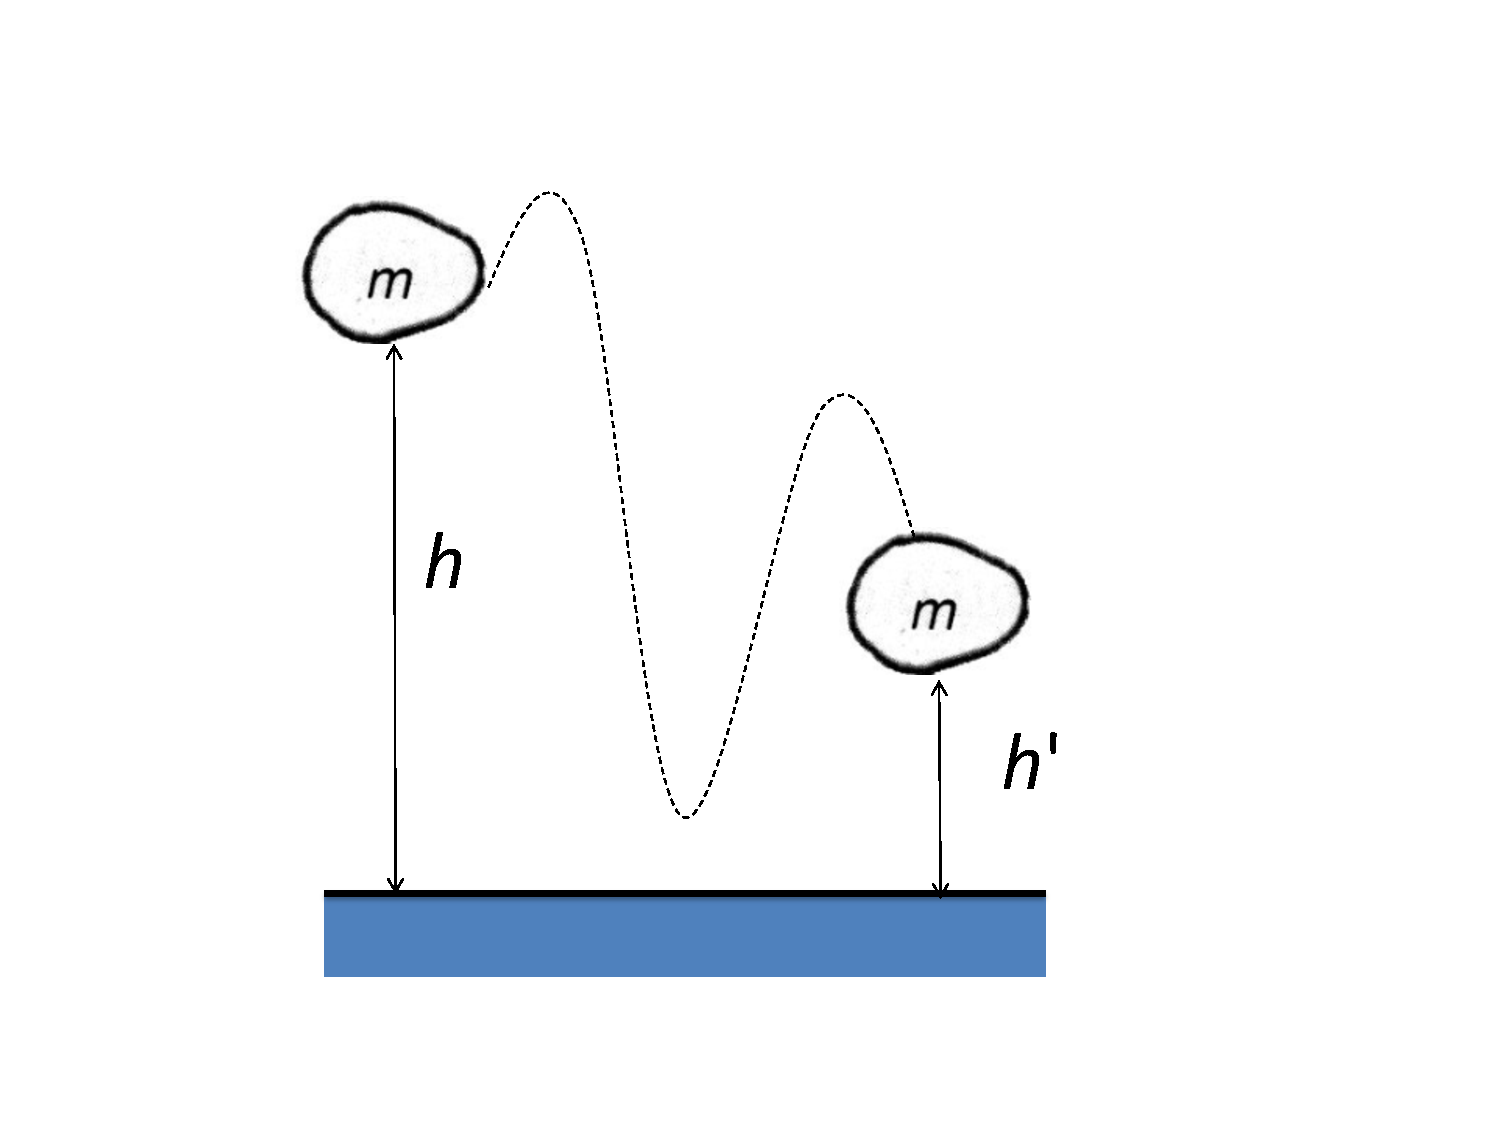
\includegraphics[scale=0.35]{img/potential-energy}
  \caption{Gravity potential energy.}
  \label{fig:potential-energy}
\end{figure}

Consider heap pop. To evaluate the cost, let the potential be $\Phi(H)$ before pop. It is the result accumulated by a series of insert and merge operations. The heap becomes $H'$ after tree consolidation. The new potential is $\Phi(H')$. The difference between $\Phi(H')$ and $\Phi(H)$, plus the cost of tree consolidation give the amortized performance. Define the potential as:

\be
\Phi(H) = t(H)
\ee

Where $t(H)$ is the number of trees in the heap. Let the upper bound of rank for all trees as $R(n)$, where $n$ is the number of elements in the heap. After tree consolidation, there are at most $t(H') = R(n) + 1$ trees. Before consolidation, there is another operation contributes to running time. we removed the root of min-tree, then add all sub-trees to the heap. We consolidate at most $R(n) + t(H) -1$ trees. Let the pop performance bound to $T$, the consolidation bound to $T_c$, the amortized time is given as below:

\be
\begin{array}{rcl}
T & = & T_c + \Phi(H') -\Phi(H) \\
  & = & O(R(n) + t(H) - 1) + (R(n) + 1) - t(H) \\
  & = & O(R(n))
\end{array}
\ee

Insert, merge, and pop ensure all trees are binomial trees, therefore, the upper bound of $R(n)$ is $O(\lg n)$.

\subsection{Increase priority}
\index{Fibonacci Heap!decrease key}

We can use heap to manage tasks with priority. When need prioritize a task, we decrease the corresponding element, making it close to the heap top. Some graph algorithms, like the minimum spanning tree and Dijkstra's algorithm rely on this heap operation\cite{CLRS} meet amortized constant time. Let $x$ be a node in the heap $H$, we need decrease its value to $k$. As shown in \cref{fig:cut-fib-tree}, if the element in $x$ is less than the one in its parent $y$, we cut $x$ off $y$, the add it the heap (forest). Although it ensures the parent still holds the minimum in the tree, it is not binomial tree any more. The performance drops when loss too many sub-trees. We add another rule to address this problem: {\em If a node losses its second sub-tree, it is immediately cut from parent, and added to the heap (forest).}

\begin{figure}[htbp]
  \centering
  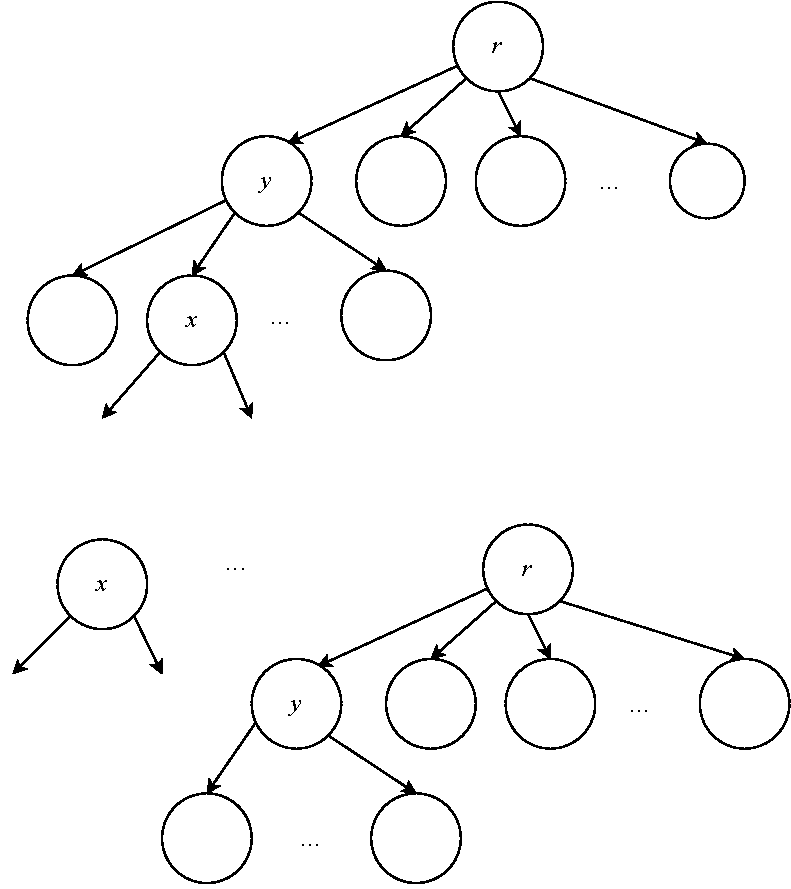
\includegraphics[scale=0.5]{img/fib-cut-past}
  \caption{If $key\ x < key\ y$, cut $x$ off and add to the heap.}
  \label{fig:cut-fib-tree}
\end{figure}

\begin{algorithmic}[1]
\Function{Decrease}{$H, x, k$}
  \State \Call{Key}{$x$} $\gets k$
  \State $p \gets $ \Call{Parent}{$x$}
  \If{$p \neq$ NIL and $k < $ \Call{Key}{$p$}}
    \State \Call{Cut}{$H, x$}
    \State \Call{Cascade-Cut}{$H, p$}
  \EndIf
  \If{$k <$ \Call{Top}{$H$}}
    \State \Call{Min-Tree}{$H$} $\gets x$
  \EndIf
\EndFunction
\end{algorithmic}

Where function \textproc{Cascade-Cut} uses a mark to record whether a node lost sub-tree before. The mark is cleared later in \textproc{Cut} function.

\begin{algorithmic}[1]
\Function{Cut}{$H, x$}
  \State $p \gets $ \Call{Parent}{$x$}
  \State remove $x$ from $p$
  \State \Call{Rank}{$p$} $\gets$ \Call{Rank}{$p$} - 1
  \State add $x$ to \Call{Trees}{$H$}
  \State \Call{Parent}{$x$} $\gets$ NIL
  \State \Call{Mark}{$x$} $\gets$ False
\EndFunction
\end{algorithmic}

During cascade cut, if node $x$ is marked, it has lost some sub-tree before. We need recursively cut along the parent till root.

\begin{algorithmic}[1]
\Function{Cascade-Cut}{$H, x$}
  \State $p \gets $ \Call{Parent}{$x$}
  \If{$p \neq$ NIL}
    \If{\Call{Mark}{$x$} $= $ False}
      \State \Call{Mark}{$x$} $\gets$ True
    \Else
      \State \Call{Cut}{$H, x$}
      \State \Call{Cascade-Cut}{$H, p$}
    \EndIf
  \EndIf
\EndFunction
\end{algorithmic}

\begin{Exercise}\label{ex:fibo-heap-decrease}
Why is \textproc{Decrease} bound to amortized $O(1)$ time?
\end{Exercise}

\begin{Answer}[ref = {ex:fibo-heap-decrease}]
Why is \textproc{Decrease} bound to amortized $O(1)$ time?

Define the potential function as:

\[
\Phi(H) = t(H) + 2m(H)
\]

Where $t(H)$ is the number of trees in the heap, and $m(H)$ is the number of the nodes being marked. As we mark, then later cut and clear the flag, its coefficient is 2. \textproc{Decrease} takes $O(1)$ time to cut $x$ off, then recursively call \textproc{Cascade-Cut}. Assume it's recursively called $c$ times. Each time takes $O(1)$ time to call \textproc{Cut}, then continue recursion. Hence the total cost of \textproc{Decrease} is $O(c)$.

For the potential change, let $H$ is the heap before we call \textproc{Decrease}, every recursive \textproc{Cascade-Cut} cuts a marked node off, then clear the flag (except for the last call). After that, there are $t(H) + c$ trees, including the original $t(H)$ trees, the cut and added back $c - 1$ trees, and the tree with $x$ as the root. There are at most $m(H) - c + 2$ marked nodes, including the original $m(H)$ nodes, minus the $c - 1$ nodes being cleared in the \textproc{Cascade-Cut} call. The last call may mark another node. The potential changes at most:

\[
t(H) + c + 2(m(H) - c + 2) - [t(H) + 2m(H)] = 4 - c
\]

Hence the amortized cost is at most $O(c) + 4 - c = O(1)$.
\end{Answer}

\subsection{The name of Fibonacci heap}

We are yet to implement \textproc{Max-Rank}($n$). It defines the upper bound of tree rank for a Fibonacci heap of $n$ elements.

\begin{lemma}
\label{lemma:Fib-degree}
For any tree $x$ in a Fibonacci Heap, let $k = rank(x)$, and $|x| = size(x)$, then

\be
  |x| \geq F_{k+2}
\ee

Where $F_k$ is the $k$-th Fibonacci number:

\[
\begin{array}{rcl}
F_0 & = & 0 \\
F_1 & = & 1 \\
F_k & = & F_{k-1} + F_{k-2} \\
\end{array}
\]
\end{lemma}

\begin{proof}
For tree $x$, let its $k$ sub-trees be $y_1, y_2, ..., y_k$, ordered by the time when they are linked to $x$. Where $y_1$ is the first, and $y_k$ is the latest. Obviously, $|y_i| \geq 0$. When link $y_i$ to $x$, there have already been sub-trees of $y_1, y_2, ..., y_{i-1}$. Because we only link nodes of the same rank, by that time we have:

\[
  rank(y_i) = rank(x) = i - 1
\]

After that, $y_i$ can lost additional sub-tree at most, (through the \textproc{Decrease}). Once loss the second sub-tree, it will be cut off then add to the forest. For any $i = 2, 3, ..., k$, we have:

\[
rank(y_i) \geq i-2
\]

Let $s_k$ be the {\em minimum possible size} of tree $x$, where $k = rank(x)$. It starts from $s_0 = 1$, $s_1 = 2$. i.e. there is at least a node in tree of rank 0, at least two nodes in tree of rank 1, at least $k$ nodes in tree of rank $k$.

\bea*{rcl}
|x| & \geq & s_k \\
    & =   & 2 + s_{rank(y_2)} + s_{rank(y_3)} + ... + s_{rank(y_k)} \\
    & \geq & 2 + s_0 + s_1 + ... + s_{k-2} \\
\eea*

The last row holds because $rank(y_i) \geq i - 2$, and $s_k$ is monotonic, hence $s_{rank(y_i)} \geq s_{i-2}$. We next show that $s_k > F_{k+2}$. Apply induction. For edge case, $s_0 = 1 \geq F_2 = 1$, and $s_1 = 2 \geq F_3 = 2$; For induction case $k \geq 2$.

\bea*{rcll}
|x| & \geq & s_k & \\
    & \geq & 2 + s_0 + s_1 + ... + s_{k-2} & \\
    & \geq & 2 + F_2 + F_3 + ... + F_k & \text{induction hypothesis}\\
    & =    & 1 + F_0 + F_1 + F_2 + ... + F_k & \text{from} F_0 = 0, F_1 = 1 \\
\eea*

Next, we prove:

\be
F_{k+2} = 1 +  \sum_{i=0}^{k} F_i
\ee

Use induction again:

\begin{itemize}
\item Edge case, $F_2 = 1 + F_0 = 2$
\item Induction case, suppose it's true for $k+1$.
\bea*{rcll}
  F_{k+2} & = & F_{k+1} + F_k & \\
         & = & (1 + \displaystyle \sum_{i=0}^{k-1}F_i) + F_k & \text{induction hypothesis} \\
         & = & 1 + \displaystyle \sum_{i=0}^{k} F_i & \\
\eea*
\end{itemize}

Wrap up to the final result:
\be
n \geq |x| \geq F_{k+2}
\ee
\end{proof}

For Fibonacci sequence, $F_k \geq \phi^k$, where $\phi = \dfrac{1+\sqrt{5}}{2}$ is the golden ratio. We prove that pop is amortized $O(\lg n)$ algorithm. We can define $maxRank$ as:

\be
  MaxRank(n) = 1 + \lfloor \log_{\phi} n \rfloor
\ee

We can also implement \textproc{Max-Degree} from Fibonacci numbers:

\begin{algorithmic}[1]
\Function{Max-Rank}{$n$}
  \State $F_0 \gets 0, F_1 \gets 1$
  \State $k \gets 2$
  \Repeat
    \State $F_k \gets F_{k_1} + F_{k_2}$
    \State $k \gets k + 1$
  \Until{$F_k < n$}
  \State \Return $k - 2$
\EndFunction
\end{algorithmic}

\section{Pairing Heaps}
\label{pairing-heap} \index{Pairing heap}

It's complex to implement Fibonacci heap. Pairing heap provides another option. It's easy to implement, and the performance is good. Most operations, like insert, top, merge are bound to constant time. the pop is conjectured to be amortized $O(\lg n)$ time\cite{pairing-heap}\cite{okasaki-book}.

\subsection{Definition}
\index{Pairing heap!definition}

A pairing heap is a multi-way tree. The root holds the minimum. A pairing heap is either empty $\nil$, or a $k$-ary tree, consists of a root and multiple sub-trees, denoted as $(x, ts)$. We can also use `left child, right sibling' way to define the tree.

\begin{Haskell}
data PHeap a = E | Node a [PHeap a]
\end{Haskell}

\subsection{Merge, insert, and top}
\index{Pairing heap!insert} \index{Pairing heap!top}

There are two cases when merge two heaps:

\begin{enumerate}
\item Either heap is $\nil$, the result is the other heap;
\item Otherwise, compare the two roots, turn the greater one as the new sub-tree of the other.
\end{enumerate}

\be
\begin{array}{rcl}
merge\ \nil\ h_2 & = & h_2 \\
merge\ h_1\ \nil & = & h_1 \\
merge\ (x, ts_1)\ (y, ts_2) & = & \begin{cases}
  x < y: & (x, (y, ts_2) : ts_1) \\
  \text{otherwise}: & (y, (x, ts1) : ts_2) \\
  \end{cases}
\end{array}
\ee

$merge$ is bound to constant time. With the `left-child, right
sibling' method, we link the heap with greater root as the first sub-tree of the other.

\begin{algorithmic}[1]
\Function{Merge}{$H_1, H_2$}
  \If{$H_1 = $ NIL}
    \State \Return $H_2$
  \EndIf
  \If{$H_2 = $ NIL}
    \State \Return $H_1$
  \EndIf
  \If{\Call{Key}{$H_2$} $<$ \Call{Key}{$H_1$}}
    \State \Call{Exchange}{$H_1 \leftrightarrow H_2$}
  \EndIf
  \State \Call{Sub-Trees}{$H_1$} $\gets$ \textproc{Link}($H_2$, \Call{Sub-Trees}{$H_1$})
  \State \Call{Parent}{$H_2$} $\gets H_1$
  \State \Return $H_1$
\EndFunction
\end{algorithmic}

Similar to Fibonacci heap, we implement insert with merge as \cref{eq:fib-insert}. We access the top element from the root: $top\ (x, ts) = x$. Both operations are bound to constant time.

\subsection{Increase priority}
\index{Pairing heap!decrease key}

When decrease the value in a node, we cut the sub-tree rooted with this node, then merge it back to the heap. If the node is the root, we can directly decrease its value.

\begin{algorithmic}[1]
\Function{Decrease}{$H, x, k$}
  \State \Call{Key}{$x$} $\gets k$
  \State $p \gets$ \Call{Parent}{$x$}
  \If{$p \neq$ NIL}
    \State Remove $x$ from \Call{Sub-Trees}{$p$}
    \State \Call{Parent}{$x$} $\gets$ NIL
    \State \Return \Call{Merge}{$H, x$}
  \EndIf
  \State \Return $H$
\EndFunction
\end{algorithmic}

\subsection{Pop}
\index{Pairing heap!pop}

After pop the root, we consolidate the remaining sub-trees to a tree:

\be
pop\ (x, ts) = \textit{consolidate}\ ts
\ee

We firstly merge every two sub-trees from left to right, then merge these paired results from right to left to a tree. This explains the why we name it `paring heap'. \Cref{fig:merge-pairs,fig:merge-right} show the paired merge.

\begin{figure}[htbp]
  \centering
  \subcaptionbox{Before pop.}{\includegraphics[scale=0.4]{img/pairing-hp}} \\
  \subcaptionbox{Pop 2, there are 9 sub-trees.}{\includegraphics[scale=0.4]{img/pairs}} \\
  \subcaptionbox{Merge with pairs, leave the last tree.}{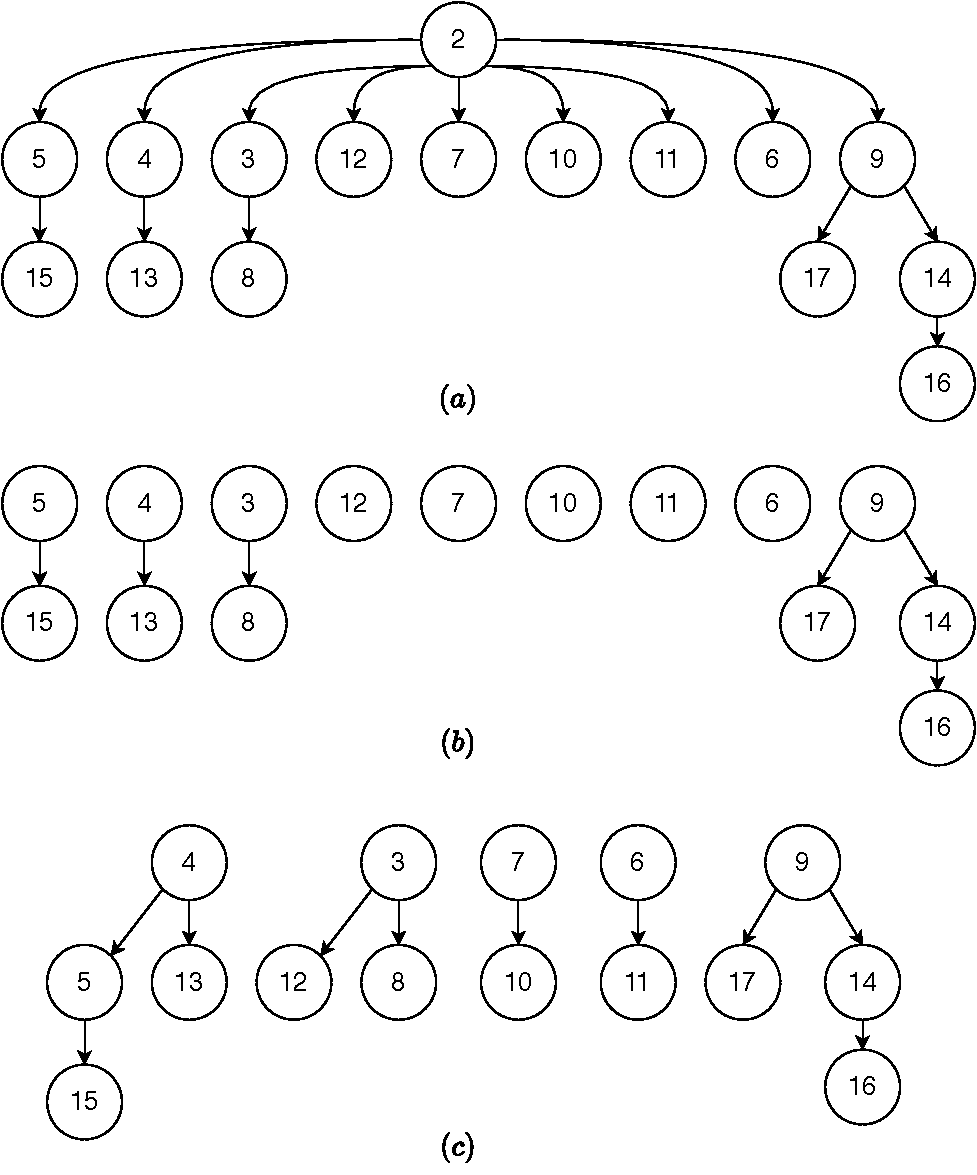
\includegraphics[scale=0.4]{img/pairs-merge}} \\
  \caption{Pop the root, merge sub-trees in pairs.}
  \label{fig:merge-pairs}
\end{figure}

\begin{figure}[htbp]
  \centering
  \subcaptionbox{Merge 9 and 6.}{\hspace{0.2\textwidth}\includegraphics[scale=0.4]{img/right-merge-1}\hspace{0.2\textwidth}}
  \subcaptionbox{Merge 7.}{\hspace{0.1\textwidth}\includegraphics[scale=0.4]{img/right-merge-2}\hspace{0.1\textwidth}} \\
  \subcaptionbox{Merge 3.}{\hspace{0.1\textwidth}\includegraphics[scale=0.4]{img/right-merge-3}\hspace{0.1\textwidth}}
  \subcaptionbox{Merge 4.}{\hspace{0.1\textwidth}\includegraphics[scale=0.4]{img/right-merge-4}\hspace{0.1\textwidth}}
  \caption{Merge from right to left.}
  \label{fig:merge-right}
\end{figure}

\be
\begin{array}{rcl}
\textit{consolidate}\ [\ ] & = & \nil \\
\textit{consolidate}\ [t] & = & t \\
\textit{consolidate}\ (t_1 : t_2 : ts) & = & merge\ (merge\ t_1\ t_2)\ (consolidate\ ts)
\end{array}
\ee

The corresponding `left child, right sibling' implementation is as below:

\begin{algorithmic}[1]
\Function{Pop}{$H$}
  \State $L \gets$ NIL
  \For{every $T_x$, $T_y$ in \Call{Sub-Trees}{$H$}}
    \State $T \gets $ \Call{Merge}{$T_x, T_y$}
    \State $L \gets$ \Call{Link}{$T, L$}
  \EndFor
  \State $H \gets$ NIL
  \For{$T$ in $L$}
    \State $H \gets $ \Call{Merge}{$H, T$}
  \EndFor
  \State \Return $H$
\EndFunction
\end{algorithmic}

We iterate to merge $T_x$, $T_y$ to $T$, and link ahead of $L$. When loop on $L$ the second time, we actually traversed from right to left. When there are odd number of sub-trees, $T_y = $ NIL at last, hence $T = T_x$ in this case.

\subsubsection{Delete}
\index{Pairing heap!delete}

To delete a node $x$, we can first decrease the value in $x$ to $-\infty$, then followed with a pop. There is an alternative method. If $x$ is the root, we pop it; otherwise, we cut $x$ off $H$, then apply pop to $x$, and merge $x$ back to $H$:

\begin{algorithmic}[1]
\Function{Delete}{$H, x$}
  \If{$H = x$}
    \State \Call{Pop}{$H$}
  \Else
    \State $H \gets$ \Call{Cut}{$H, x$}
    \State $x \gets$ \Call{Pop}{$x$}
    \State \Call{Merge}{$H, x$}
  \EndIf
\EndFunction
\end{algorithmic}

As delete is implemented with pop, the performance is conjectured to be amortized $O(\lg n)$ time.

\begin{Exercise}\label{ex:pairing-heap-del}
\Question{If continuously insert $n$ elements then followed with a pop. The performance overhead is big when $n$ is a large number (although the amortized performance is $O(\lg n)$. How to mitigate such worst case?}
\Question{Implement delete operation for the pairing heap.}
\Question{Implement priority change for the pairing heap, i.e. \textproc{Decrease-Key}.}
\end{Exercise}

\begin{Answer}[ref = {ex:pairing-heap-del}]
\Question{If continuously insert $n$ elements then followed with a pop. The performance overhead is big when $n$ is a large number (although the amortized performance is $O(\lg n)$. How to mitigate such worst case?

We can set a threshold $m$ to the number of sub-trees. When insert, we check whether it exceeds $m$, if yes, then perform a pop then add the element back.

\begin{Bourbaki}
MAX_SUBTREES = 16

Node<K> insert(Node<K> h, K x) {
    if h != null and length(h.subTrees) > MAX_SUBTREES {
        h = insert(pop(h), top(h))
    }
    return merge(h, Node(x))
}
\end{Bourbaki}
}

\Question{Implement delete operation for the pairing heap.

We add a parent reference to the node definition:
\begin{Bourbaki}
data Node<K> {
    K key
    Node<K> parent = null
    [Node<K>] subTrees = []

    Node<K>(K k) { key = k }
}
\end{Bourbaki}

When delete element $x$, we first lookup the heap $h$ to find the sub-tree $t$ rooted at $x$. If $t$ is the root of $h$, then we merely do a $pop$; otherwise, we get the parent $p$ of $t$, remove $t$ from its sub-trees. Then apply $pop$, and finally merge $pop(t)$ back with $h$.

\begin{Bourbaki}
Node<K> delete(Node<K> h, K x) {
    var tr = lookuptr(h, x)
    if tr == null then return h
    if tr == h then return pop(h)
    tr.parent.subtrees.remove(tr)
    tr.parent = null
    return merge(pop(tr), h)
}

Node<K> lookuptr(Node<K> h, K x) {
    if h.key == x then return h
    for var t in h.subtrees {
        var tr = lookuptr(t, x)
        if tr != null then return tr
    }
    return null
}
\end{Bourbaki}

The recursive lookup takes $O(n)$ time, where $n$ is the number of elements in the heap. Then it takes $O(m)$ time to remove $t$ from the sub-trees. The total performance is $O(n)$.
}

\Question{Implement priority change for the pairing heap, i.e. \textproc{Decrease-Key}.

If decrease the key of the root of $h$, we can directly update the key to $x$; otherwise, we get the parent of $tr$, then cut $tr$ off from the sub-trees; update the key of $tr$ to $x$, then merge $tr$ back to $h$:

\begin{Bourbaki}
Node<K> decreaseKey(Node<K> h, Node<K> tr, K x) {
    if tr == null or tr.key < x then return h
    tr.key = x
    if tr == h then return h
    tr.parent.subtrees.remove(tr)  // O(m), where m = length(subtrees)
    tr.parent = null
    return merge(tr, h)
}
\end{Bourbaki}

When use, we first call $lookuptr(h, y)$ to find the node, then update from $y$ to $x$, i.e., $deceaseKey(h, lookuptr(h, y), x)$. The performance is as same as delete, which is $O(n)$.
}
\end{Answer}

\section{Summary}

In this chapter, we extend the heap from binary tree based implementation to more data structures. Binomial heap and Fibonacci heap use forest of multi-way trees, pairing heap use a single multi-way tree.It's a common practice to post pone some expensive operation, and obtain better amortized performance.

\section{Appendix - example programs}

Definition of multi-way tree (left child, right sibling):

\begin{lstlisting}[language = Bourbaki]
data Node<K> {
    Int rank
    K key
    Node<K> parent, subTrees, sibling,
    Bool mark

    Node(K x) {
        key = x
        rank = 0
        parent = subTrees = sibling = null
        mark = false
    }
}
\end{lstlisting}

Link binomial trees:

\begin{lstlisting}[language = Bourbaki]
Node<K> link(Node<K> t1, Node<K> t2) {
    if t2.key < t1.key then (t1, t2) = (t2, t1)
    t2.sibling = t1.subTrees
    t1.subTrees = t2
    t2.parent = t1
    t1.rank = t1.rank + 1
    return t1
}
\end{lstlisting}

Binomial heap insert:

\begin{lstlisting}[language = Bourbaki]
Node<K> insert(K x, Node<K> h) = insertTree(Node(x), h)

Node<K> insertTree(Node<K> t, Node<K> h) {
    var h1 = Node()
    var prev = h1
    while h != null and h.rank <= t.rank {
        var t1 = h
        h = h.sibling
        if t.rank == t1.rank {
            t = link(t, t1)
        } else {
            prev.sibling = t1
            prev = t1
        }
    }
    prev.sibling = t
    t.sibling = h
    return removeFirst(h1)
}

Node<K> removeFirst(Node<K> h) {
    var next = h.sibling
    h.sibling = null
    return next
}
\end{lstlisting}

Binomial heap recursive insert:

\begin{Haskell}
data BiTree a = Node { rank :: Int
                     , key :: a
                     , subTrees :: [BiTree a]}

type BiHeap a = [BiTree a]

link t1@(Node r x c1) t2@(Node _ y c2) =
    if x < y then Node (r + 1) x (t2:c1)
    else Node (r + 1) y (t1:c2)

insertTree t [] = [t]
insertTree t ts@(t':ts') | rank t < rank t' = t:ts
                         | rank t > rank t' = t' : insertTree t ts'
                         | otherwise = insertTree (link t t') ts'

insert x = insertTree (Node 0 x [])
\end{Haskell}

Binomial heap merge:

\begin{lstlisting}[language = Bourbaki]
Node<K> merge(h1, h2) {
    var h = Node()
    var prev = h
    while h1 != null and h2 != null {
        if h1.rank < h2.rank {
            prev.sibling = h1
            prev = prev.sibling
            h1 = h1.sibling
        } else if h2.rank < h1.rank {
            prev.sibling = h2
            prev = prev.sibling
            h2 = h2.sibling
        } else {
            var (t1, t2) = (h1, h2)
            (h1, h2) = (h1.sibling, h2.sibling)
            h1 = insertTree(link(t1, t2), h1)
    }
    if h1 != null then prev.sibling = h1
    if h2 != null then prev.sibling = h2
    return removeFirst(h)
}
\end{lstlisting}

Binomial heap recursive merge:

\begin{Haskell}
merge ts1 [] = ts1
merge [] ts2 = ts2
merge ts1@(t1:ts1') ts2@(t2:ts2')
    | rank t1 < rank t2 = t1:(merge ts1' ts2)
    | rank t1 > rank t2 = t2:(merge ts1 ts2')
    | otherwise = insertTree (link t1 t2) (merge ts1' ts2')
\end{Haskell}

Binomial tree pop:

\begin{lstlisting}[language = Bourbaki]
Node<K> reverse(Node<K> h) {
    Node<K> prev = null
    while h != null {
        var x = h
        h = h.sibling
        x.sibling = prev
        prev = x
    }
    return prev
}

(Node<K>, Node<K>) extractMin(Node<K> h) {
    var head = h
    Node<K> tp = null
    Node<K> tm = null
    Node<K> prev = null
    while h != null {
        if tm == null or h.key < tm.key {
            tm = h
            tp = prev
        }
        prev = h
        h = h.sibling
    }
    if tp != null {
        tp.sibling = tm.sibling
    } else {
        head = tm.sibling
    }
    tm.sibling = null
    return (tm, head)
}

(K, Node<K>) pop(Node<K> h) {
    var (tm, h) = extractMin(h)
    h = merge(h, reverse(tm.subtrees))
    tm.subtrees = null
    return (tm.key, h)
}
\end{lstlisting}

Binomial heap recursive pop:

\begin{Haskell}
pop h = merge (reverse $ subTrees t) ts where
    (t, ts) = extractMin h

extractMin [t] = (t, [])
extractMin (t:ts) = if key t < key t' then (t, ts)
                    else (t', t:ts') where
    (t', ts') = extractMin ts
\end{Haskell}

Merge Fibonacci heaps with bidirectional linked list:

\begin{lstlisting}[language = Bourbaki]
FibHeap<K> merge(FibHeap<K> h1, FibHeap<K> h2) {
    if isEmpty(h1) then return h2
    if isEmpty(h2) then return h1
    FibHeap<K> h = FibHeap<K>()
    h.trees = concat(h1.trees, h2.trees)
    h.minTree = if h1.minTree.key < h2.minTree.key
                then h1.minTree else h2.minTree
    h.size = h1.size + h2.size
    return h
}

bool isEmpty(FibHeap<K> h) = (h == null or h.trees == null)

Node<K> concat(Node<K> first1, Node<K> first2) {
  var last1 = first1.prev
  var last2 = first2.prev
  last1.next = first2
  first2.prev = last1
  last2.next = first1
  first1.prev = last2
  return first1
}
\end{lstlisting}

Consolidate trees in Fibonacci heap:

\begin{Haskell}
consolidate = foldr melt [] where
    melt t [] = [t]
    meld t (t':ts) | rank t == rank t' = meld (link t t') ts
                   | rank t <  rank t' = t : t' : ts
                   | otherwise = t' : meld t ts
\end{Haskell}

Consolidate trees with auxiliary array:

\begin{lstlisting}[language = Bourbaki]
void consolidate(FibHeap<K> h) {
    Int R = maxRank(h.size) + 1
    Node<K>[R] a = [null, ...]
    while h.trees != null {
        var x = h.trees
        h.trees = remove(h.trees, x)
        Int r = x.rank
        while a[r] != null {
            var y = a[r]
            x = link(x, y)
            a[r] = null
            r = r + 1
        }
        a[r] = x
    }
    h.minTr = null
    h.trees = null
    for var t in a if t != null {
        h.trees = append(h.trees, t)
        if h.minTr == null or t.key < h.minTr.key then h.minTr = t
    }
}
\end{lstlisting}

Fibonacci heap pop:

\begin{Haskell}
pop (FH _ (Node _ x []) []) = (x, E)
pop (FH sz (Node _ x tsm) ts) = (x, FH (sz - 1) tm ts') where
    (tm, ts') = extractMin $ consolidate (tsm ++ ts)
\end{Haskell} %$

Decrease value in Fibonacci heap:

\begin{lstlisting}[language = Bourbaki]
void decrease(FibHeap<K> h, Node<K> x, K k) {
    var p = x.parent
    x.key = k
    if p != null and k < p.key {
        cut(h, x)
        cascadeCut(h, p)
    }
    if k < h.minTr.key then h.minTr = x
}

void cut(FibHeap<K> h, Node<K> x) {
    var p = x.parent
    p.subTrees = remove(p.subTrees, x)
    p.rank = p.rank - 1
    h.trees = append(h.trees, x)
    x.parent = null
    x.mark = false
}

void cascadeCut(FibHeap<K> h, Node<K> x) {
    var p = x.parent
    if p == null then return
    if x.mark {
        cut(h, x)
        cascadeCut(h, p)
    } else {
        x.mark = true
    }
}
\end{lstlisting}

\section{Answers}
\shipoutAnswer

\ifx\wholebook\relax \else
\begin{thebibliography}{99}

\bibitem{K-ary-tree}
K-ary tree, Wikipedia. \url{https://en.wikipedia.org/wiki/K-ary_tree}

\bibitem{CLRS}
Thomas H. Cormen, Charles E. Leiserson, Ronald L. Rivest and Clifford Stein. ``Introduction to Algorithms, Second Edition''. The MIT Press, 2001. ISBN: 0262032937.

\bibitem{okasaki-book}
Chris Okasaki. ``Purely Functional Data Structures''. Cambridge university press, (July 1, 1999), ISBN-13: 978-0521663502

\bibitem{wiki-pascal-triangle}
Wikipedia, ``Pascal's triangle''. \url{https://en.wikipedia.org/wiki/Pascal's_triangle}

\bibitem{hackage-fibq}
Hackage. ``An alternate implementation of a priority queue based on a Fibonacci heap.'', \url{http://hackage.haskell.org/packages/archive/pqueue-mtl/1.0.7/doc/html/src/Data-Queue-FibQueue.html}

\bibitem{okasaki-fibh}
Chris Okasaki. ``Fibonacci Heaps.'' \url{http://darcs.haskell.org/nofib/gc/fibheaps/orig}

\bibitem{pairing-heap}
Michael L. Fredman, Robert Sedgewick, Daniel D. Sleator, and Robert E. Tarjan. ``The Pairing Heap: A New Form of Self-Adjusting Heap'' Algorithmica (1986) 1: 111-129.

\end{thebibliography}

\expandafter\enddocument
\fi
